\documentclass[conference]{IEEEtran}

\usepackage{cite}
\usepackage{amsmath,amssymb,amsfonts}
\usepackage{algorithmic}
\usepackage{graphicx}
\usepackage{textcomp}
\usepackage{xcolor}


\usepackage{times}
%\usepackage{ulem}
% (Note: If you have the commercial package `mathtime,' (from
% y&y (http://www.yandy.com), it is much better, but the `times'
% package works too). So, if you have it...
%\usepackage{mathtime}
\usepackage[mediumspace,mediumqspace,Gray,squaren]{SIunits}
% \usepackage{amssymb}
\usepackage[cmex10]{amsmath}
% \usepackage{amsfonts}

% \usepackage{color}
%\usepackage{xcolor,soul}
%Use for Hightlighting

% This is for Sub-figures
\usepackage[hang,center,tight]{subfigure}
\usepackage{float}
\usepackage{graphicx}

% This is for Graphic
%\usepackage[pdftex]{graphicx}

% This is for citation
\usepackage[hyphens,obeyspaces]{url}
\usepackage{cite}
\usepackage[none]{hyphenat}
%\usepackage{caption}
\tolerance=9999
\emergencystretch=10pt
\hyphenpenalty=10000
\exhyphenpenalty=100

\usepackage{booktabs}
\usepackage{textgreek}

% This is for Table Package
%\usepackage{tabu}
\usepackage{booktabs}
\usepackage{threeparttable}
\usepackage{multirow}

% Hyper Extension
%\usepackage[none]{hyphenat}

% LaTeX the ability to create hyperlinks within the document
%\usepackage[colorlinks=false,hidelinks]{hyperref}

% for any plug-in code... insert it here. For example, the CDC style...
%\usepackage{ieeecdc}

%\usepackage{ifthen}
%\newboolean{includefigs}
%\setboolean{includefigs}{false}
%\newcommand{\condcomment}[2]{ifthenelse{#1}{#2}{}}
%\input{endpics} % endpics.tex includes all the figures and tables

% This is for Algorithm Writing
\usepackage{algorithm}
\usepackage{algorithmic}
% \usepackage{algpseudocode}
\renewcommand{\algorithmicrequire}{\textbf{Input:}}
\renewcommand{\algorithmicensure}{\textbf{Output:}}
\renewcommand{\algorithmiccomment}[1]{/* #1 */}

\newtheorem{definition}{\textbf{Definition}}
\newtheorem{problem}{\textbf{Problem}}
\newcommand{\prob}[2]{\begin{problem}[#1] #2 \end{problem}}
\newtheorem{scenario}{\textbf{Scenario}}
\newcommand{\scen}[2]{\begin{scenario}[#1] #2 \end{scenario}}

\usepackage{textcomp} % \textmu \textohm
%\usepackage{fixltx2e} % \textsuperscript

%\ This is for comment
\usepackage{verbatim}

\usepackage{lineno}
%\linenumbers

\usepackage [english]{babel}
\usepackage{blindtext}
\pagestyle{empty}

%\newcommand{\upcite}[1]{\textsuperscript{\textsuperscript{\cite{#1}}}}
\begin{document}
\bstctlcite{IEEEexample:BSTcontrol}
\graphicspath{{./figures/}{./biography/}{./}}

%----------------------------------------------------------------------
% Title Information, Abstract and Keywords
%-----------------------------------------------
\title{SpiceModelIR: Cross-Simulator SPICE Translation via Semantic IR and Intelligent Parameter Inference}

% rmb to comment this for apccas submission
% \author{
% Shen Ni Lee$^{1,2}$,
% Haochen Du$^{1}$,
% Kian Kit Cheah$^{1,2}$,
% Chao Wang$^{1}$,
% Kainlu Low$^{1}$, \\
% Harikrishnan Ramiah$^{2,}$*, and
% Yongfu Li$^{1,3,}$* \\
% 1. School of Integrated Circuits, Shanghai Jiao Tong University, Shanghai, China. \\
% 2. Department of Electrical Engineering, University of Malaya, Malaysia. \\
% \thanks{
% This work is supported in part by the National Natural Science Foundation of China under Grants No. 62350610271 and 62201340, and in part by the Explorers Program of Shanghai (Basic Research Funding) under Grant No. 24TS140020.
% The corresponding authors are 
% Harikrishnan Ramiah (hrkhari@um.edu.my), and
% Yongfu Li (yongfu.li@sjtu.edu.cn).}
% }

\maketitle

\begin{abstract}
Till today, semiconductor design workflows still face significant interoperability challenges due to incompatible SPICE files, primarily across Cadence Spectre, Synopsys HSPICE, and Berkeley ngspice. Manual translation is labor-intensive, error-prone, and typically lacks comprehensive validation. This paper presents SpiceModelIR, a semantic translation framework that enables the automated, bidirectional conversion of device model libraries across these formats. Unlike conventional syntax-based tools, SpiceModelIR utilizes a device-physics-aware intermediate representation (IR) paired with an intelligent parameter inference system that automatically populates missing process-dependent variables with physically sensible defaults. To ensure electrical correctness, the framework integrates a multi-mode verification suite that encompasses DC, AC, transient, sanity, Monte Carlo, and round-trip checks. Evaluated on 15 process design kits (PDKs) comprising 322 source files, SpiceModelIR successfully generated 6,638 translated models and achieved a 100 percent pass rate across 587 full-mode verification tests. By condensing PDK porting efforts from hundreds of engineer-hours to mere seconds, SpiceModelIR establishes a robust, reproducible workflow for cross-simulator model portability.
\end{abstract}

\begin{IEEEkeywords}
SPICE simulation, model translation, format conversion, parameter mapping, closed-loop validation, semiconductor design automation, intermediate representation.
\end{IEEEkeywords}

\section{Introduction}
\label{sec:introduction}
%----------------------------------------------------------------------
%---------------------------------------------------------------------
%What is the problem? Use 3 sentences to complete the introduction paragraph and end the paragraph with a statement. E.g. Precise temperature measuring is one of the demanding application from all the health monitoring application in IoT wearable devices.
%---------------------------------------------------------------------

\IEEEPARstart{W}{hile} SPICE simulation is used extensively in the semiconductor design industry for circuit verification and optimization \cite{Pratap_2014, Kundert_1995, Vogt_ngspice, a2024_single}, the fragmentation of simulator formats, such as Cadence Spectre, Synopsys HSPICE, and Berkeley ngspice, creates significant interoperability bottlenecks \cite{Chhabria_2025, Goldman_2000}. Divergent syntax and parameter conventions force design teams into error-prone manual translation, consuming hundreds of engineer-hours per technology node \cite{Dahad_2021, spiceerror, engineererror, a2024_kb}. Existing structural parsers successfully map Verilog to Verilog-A, but target behavioral bridging rather than transistor-level SPICE portability \cite{Shao_2023_V2Va, Wang_2024_V2VaPlus}.

A second critical challenge emerges from missing process-dependent parameters. When foundries distribute PDKs, they often split transistor models from their corner-variation definition files. Variables like \texttt{tox\_default} or \texttt{u0\_n} vanish during translation, leaving unresolved symbols that crash simulators or corrupt numerical behavior (e.g., zero-initialization of oxide thickness causes immediate division-by-zero errors). LLMs have recently advanced datasheet extraction, netlist curation, and code synthesis \cite{Chen_2025_D2S, Chen_2024_DocEDA, Bhandari_2024, Vungarala_2024_SPICEPilot}, yet they target initial netlist generation rather than the precise parameter recovery required for cross-dialect translation. Generic netlist rewriters \cite{DallOra_2025} lack the semantic and physics grounding to handle these dependencies consistently. As a result, teams still resort to manual model porting, proprietary tool lock-in, and expensive re-validation cycles \cite{Zhu_2012, spicesec2025}.

To address these limitations, this paper introduces SpiceModelIR, automating SPICE translation via a semantic pipeline grounded in classical device physics \cite{Vladimirescu_1994, Tuinenga_1995, Tsividis_2011, Sze_2007, Baker_2010, Rabaey_2003, Lee_2004, Mead_1980, Cheng_1999_MOSFET, Chauhan_BSIMCMG_2020}. SpiceModelIR integrates: (1) a physics-aware intermediate representation (IR) capturing dialect-independent semantics; (2) an intelligent parameter inference system assigning physically sensible defaults to missing parameters; and (3) an automated, multi-mode verification pipeline. Utilizing a constraint-aware verifier to filter known BSIM4 limitations, this framework ensures robust functional equivalence, achieving a perfect pass rate of 587/587 across 15 PDKs.

% --- Concrete example added for clarity ---
\begin{center}
\textbf{Concrete translation example (illustrative).}
\end{center}
Below is a minimal example of a translation-blocking issue. The model references undefined corner parameters that cause simulator crashes without resolution.
\begin{center}
\small
\begin{minipage}{0.85\columnwidth}
\texttt{\% Before (HSPICE with unresolved symbols)}\\
\texttt{.model M1 NMOS (vth=\{tox\_default\} u0=\{u0\_n\})}\\[0.3em]
\texttt{\% After (ngspice-ready, inferred defaults)}\\
\texttt{.model M1 NMOS (vth=0.35 u0=0.03)}
\end{minipage}
\end{center}

The example above is intentionally small: it demonstrates an undefined-symbol failure that a syntax-only rewriter would leave unresolved (producing a runtime simulator error), whereas SpiceModelIR resolves the missing symbols with physics-grounded baselines and emits a simulator-acceptable model.

\section{The Cross-Simulator Translation Problem}
\label{sec:problem}

\subsection{Real-world barriers}
Production PDKs do not differ only in keyword spelling. The deeper barriers are parameter dependencies, equation parsing rules, and BSIM model constraints. A typical scenario: a 180~nm commercial PDK distributes transistor models separately from corner-variation files. When teams port these to a different simulator, they face multiple failures that syntax-alone cannot resolve.

\paragraph{Missing symbolic parameters} crash simulations. If a netlist contains \texttt{vth0=\{tox\_default\}} but the corner file is omitted, a naive parser leaves the symbol unresolved. Worse, if the target tool zero-initializes it, oxide thickness becomes zero, triggering division-by-zero in MOSFET equations. This is a semantic failure, not a syntactic one.

\paragraph{BSIM level mismatch} blocks translation. HSPICE uses level 54 for BSIM4; ngspice uses level 14. Copying level 54 into ngspice produces a rejection. A translator must recognize both refer to the same physics and remap them.

\paragraph{Expression syntax} varies. Spectre allows ternary operators and function calls (\texttt{(cond) ? val1 : val2}, \texttt{exp(param)}); HSPICE and ngspice reject them. A correct translator normalizes the algebraic intent and emits target-compatible code.

\paragraph{Include paths} break during migration. Models reference corner files via relative paths that fail when file systems change. Text replacement alone cannot recover the missing definitions.

These six issues (undefined symbols, BSIM levels, expression syntax, include paths, non-model wrappers, simulator guardrails) affect 339 models across 15 PDKs. A successful system must solve all six.

\section{System Architecture}
\label{sec:architecture}
%==============================================================================

\begin{figure}[!t]
\centering
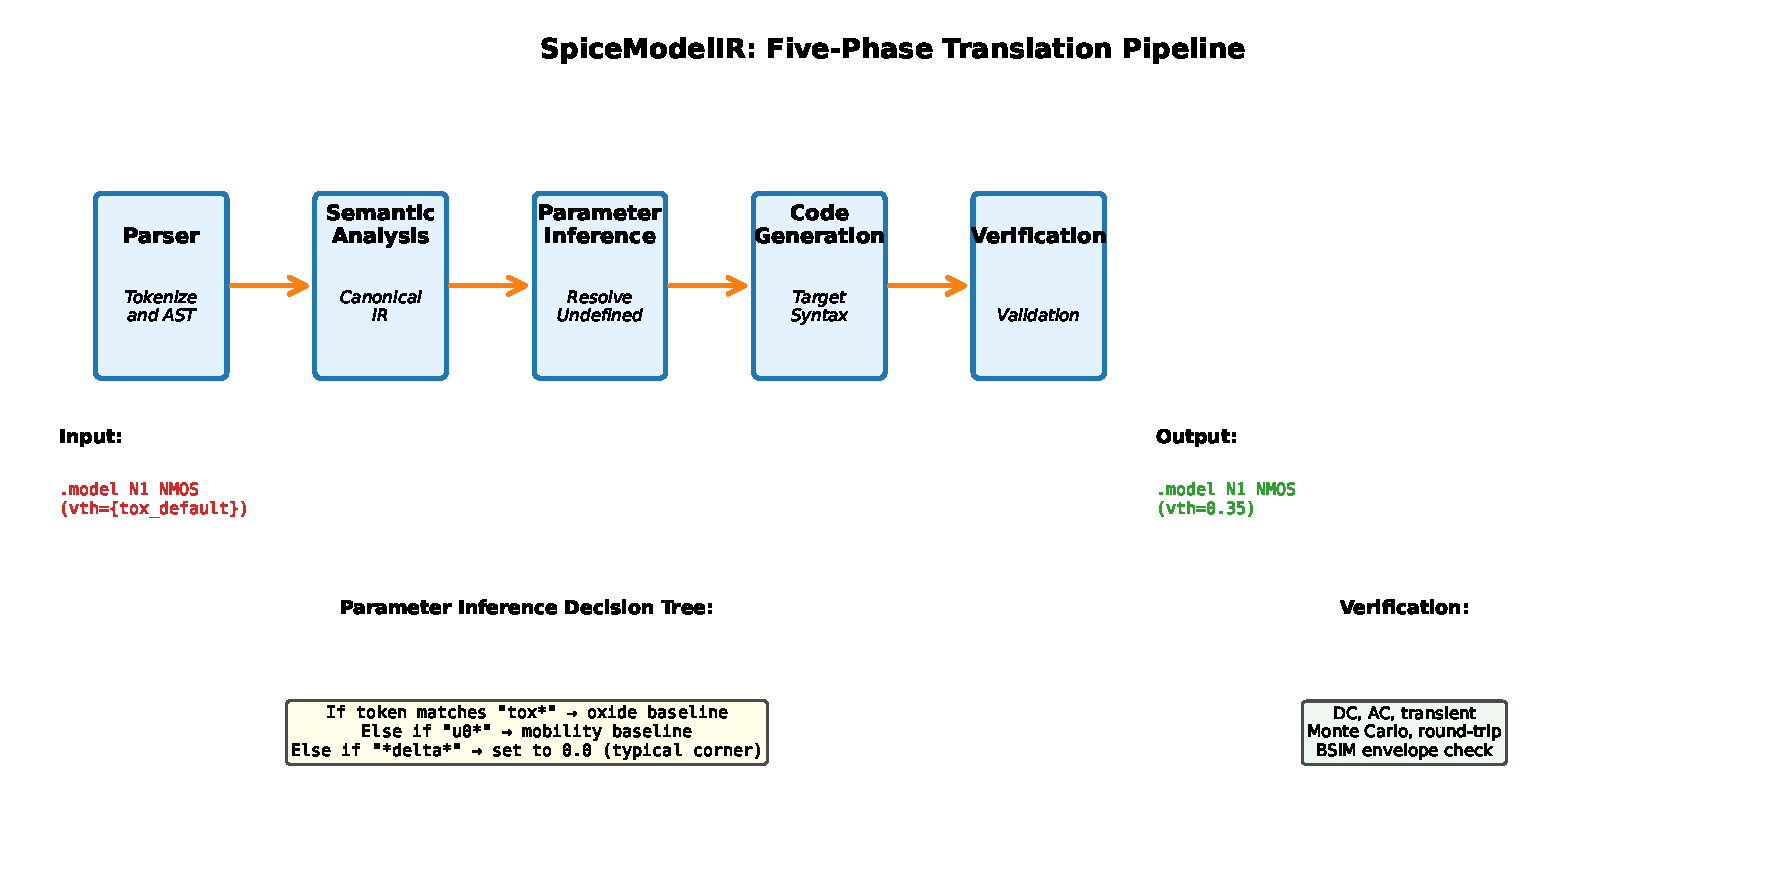
\includegraphics[width=\columnwidth]{fig_architecture.pdf}
\caption{The complete SpiceModelIR system architecture. (A) Five-phase compiler-inspired pipeline. (B) Parameter inference decision tree with regex-based token matching. (C) Constraint-aware verification filter that isolates simulator limits from translation errors.}
\label{fig:system_architecture}
\end{figure}

SpiceModelIR implements a modular, compiler-inspired architecture encompassing five sequential phases: parsing, semantic analysis, parameter inference, code generation, and verification, as illustrated in Fig. \ref{fig:system_architecture}. The core innovation is decomposing translation into three separate tasks: semantic normalization, physics-aware parameter completion, and verification. This approach is necessary because a direct text rewrite can preserve tokens while still breaking the model, as production libraries differ not only in keyword spelling but also in include structure, parameter naming, and the treatment of corner-dependent symbols. By separating the tasks of preserving model meaning, repairing undefined process-dependent values, and proving correctness, the framework remains robust on heterogeneous industrial libraries where syntax-only conversion is insufficient.

\begin{table*}[!t]
\caption{Critical Syntactic and Semantic Differences Across HSPICE, Spectre, and ngspice --- and How SpiceModelIR Resolves Them}
\label{tab:critical_diffs}
\centering
\renewcommand{\arraystretch}{1.15}
\footnotesize
\begin{tabular}{@{}p{1.6cm}p{2.0cm}p{2.0cm}p{2.0cm}p{3.0cm}@{}}
\toprule
\textbf{Issue} & \textbf{HSPICE} & \textbf{Spectre} & \textbf{ngspice} & \textbf{Solution} \\
\midrule
\multicolumn{5}{l}{\textit{\textbf{Model Declaration and Syntax}}} \\
\midrule
Model Declaration & \texttt{.model nch NMOS level=54} & \texttt{model nch nmos type=n} & \texttt{.model nch NMOS level=14} & Canonical BSIM level mapping (level 54 $\rightarrow$ 14) \\
Line Continuation & \texttt{+} at column 6 (strict) & Implicit breaks & \texttt{+} anywhere & Parser absorbs rules into AST; IR normalizes \\
Expression Parsing & Basic arithmetic & Full algebraic + ternary & Basic arithmetic & Canonicalize expressions; verify target support \\
\midrule
\multicolumn{5}{l}{\textit{\textbf{Parameters and Undefined References}}} \\
\midrule
Symbolic Params & \texttt{\{tox\}} via .param or .include & \texttt{\{tox\}} or bare & \texttt{\{tox\}} & Detect undefined; classify by pattern; apply physics baselines \\
Corner Params & External files; often omitted & External files; often omitted & External files; often omitted & Inference engine: regex match + corpus lookup + physics defaults \\
Process Variation & Delta params like \texttt{delvto} & Delta params like \texttt{delvto} & Delta params like \texttt{delvto} & Classify tokens; deltas $\rightarrow$ 0.0 (typical); scaling $\rightarrow$ 1.0 \\
\midrule
\multicolumn{5}{l}{\textit{\textbf{BSIM and Geometry}}} \\
\midrule
BSIM Levels & Level 54 (BSIM4), 49 (BSIM3v3) & Level 7 or descriptive & Level 14 (BSIM4), 8 (BSIM3) & Map to canonical IR; verify target support \\
BSIM Envelopes & Enforced; may reject at runtime & Enforced; may reject & Enforced; stricter & Constraint-aware filter: separate guardrails from true errors \\
\midrule
\multicolumn{5}{l}{\textit{\textbf{Hierarchies and Includes}}} \\
\midrule
Includes & \texttt{.include}, \texttt{.lib/.endl} sections & \texttt{section} blocks & \texttt{.include} (flat) & Flatten chains; resolve paths; substitute inferred params \\
\bottomrule
\end{tabular}
\end{table*}

The \textbf{parsing phase} begins the pipeline by separating simulator-specific syntax from the underlying model content. Spectre, HSPICE, and ngspice encode electrical intent through different continuation rules, expression syntax, sectioning styles, and wrapper structures. Parsing each dialect into an abstract syntax tree (AST) eliminates formatting noise that masks semantic mismatches. This prevents a common pitfall: a line-by-line rewriter that preserves tokens while breaking physics. Each parser handles dialect-specific syntax: HSPICE model blocks, Spectre section delimiters, and ngspice netlist syntax. The parser output consists of format-agnostic ASTs representing model structure independent of the source dialect.

Next, ASTs are normalized into a canonical intermediate representation (IR) in the \textbf{semantic analysis phase}, which extracts true physical meaning and moves the framework beyond shallow token-for-token substitution. The semantic IR reduces parsed models to their core physics. It maps device types and translates BSIM level numbers to a canonical form (e.g., HSPICE level 54 and ngspice level 14 both become BSIM4 in the IR). Additionally, the IR normalizes dialect-specific algebraic expressions and maps internal parameter relationships, clearly separating scaling factors, delta variations, and critical physics values. Finally, it embeds essential constraint metadata, including geometric limits and parameter bounds, to preserve computational accuracy and enable robust cross-dialect validation. This representation serves as the precise point where equivalent constructs from different simulators are aligned before any target-specific rewriting, ensuring the underlying executable semantics are strictly preserved.

The \textbf{parameter inference phase} tackles the hardest problem: recovering missing process-dependent parameters. When corner-variation files are unavailable (a common real-world scenario), variables like \texttt{tox\_default} become undefined. A parser-only approach leaves these symbols unresolved or zeroes them, causing simulation crashes. Instead, SpiceModelIR detects undefined tokens and assigns physics-grounded defaults. The resolution strategy combines three mechanisms. First, regex-based pattern matching recognizes token names like \texttt{tox*}, \texttt{u0*}, or \texttt{*delta*}, inferring their physical meaning. Second, corpus scanning looks at other model files in the same PDK to extract typical values. Third, the system applies device-physics baselines:
\begin{itemize}
    \item \textbf{Scaling factors} such as \textit{rhouo\_eff} and \textit{vsat\_eff} default to 1.0 to preserve nominal device characteristics.
    \item \textbf{Delta parameters} for process variation like \textit{delvto} default to 0.0, simulating a typical-typical manufacturing corner.
    \item \textbf{Critical BSIM parameters} receive standard physical baselines derived from semiconductor physics, including oxide thickness (2.5 nm), carrier mobility ($0.03 \text{ m}^2/(\text{V}\cdot\text{s})$), and threshold voltage (0.35 V).
    % (0.03 m$^2$/V·s), and threshold voltage (0.35 V).
    \item \textbf{Device-specific variants} including \textit{u0\_n18} are identified via regular expression pattern matching, enabling accurate assignments even for proprietary parameter names.
\end{itemize}

The \textbf{code generation phase} walks the IR and emits target-specific syntax. Unlike template-based rewriting, this phase actively handles BSIM level remapping and adapts expressions to the target dialect. For instance, a Spectre three-terminal capacitor is structurally converted into a target-compatible subcircuit containing parasitic capacitances. The generator concurrently handles precise device type classification and embeds the inferred parameter defaults directly into the target syntax. Finally, to ensure strict structural integrity, the resulting code is validated through native netlist parsing prior to final output.

\subsection{Closed-loop Verification System}

Translated models undergo DC, AC, and transient round-trip checks to establish strict functional equivalence. A central part of this phase is the \textbf{Constraint-Aware Filter}, which handles backend simulator guardrails \textbf{[P6]}. Ngspice often rejects models that violate the BSIM4 minimum channel length ($L_{min}$). Those rejections reflect simulator-specific limits rather than translation mistakes.

The closed-loop verification system validates translated models by running electrical tests across multiple modes and by classifying simulator failures with a compact, auditable rule base. The process has three stages. First, the log extractor collects the relevant lines from simulator standard output and standard error. Next, the normalizer converts those lines into canonical tokens such as MISSING\_SYMBOL, GEOMETRY\_VIOLATION, EXPR\_PARSE\_ERROR, and NONCONVERGENCE\_NUMERIC. Finally, the classifier evaluates the tokens against a fixed set of 32 pattern-matching rules. The rule base is intentionally compact so that each rule can be reviewed by hand. Based on the matched rule, the classifier assigns one of three labels, namely simulator-guardrail, translator-defect, or non-critical.

The rule base is designed to keep every decision auditable and reproducible. Each rule maps a standardized token pattern to a response protocol defined by its label. When the classifier returns \textit{simulator-guardrail}, the verifier logs the boundary constraint and suggests a remediation, such as increasing device dimensions or marking the model as out of envelope. When the classifier returns \textit{translator-defect}, the pipeline performs a closed-loop repair before translation is run again. That repair may rebuild include paths, infer missing parameters, or standardise expressions. When the classifier returns \textit{non-critical}, the system records the event and keeps the generated model, with the option to rerun the simulation using adjusted solver tolerances.

Representative examples of rules and the responses they trigger:
\begin{itemize}
    \item \texttt{GEOMETRY\_MIN\_VIOLATION} (\textit{simulator-guardrail}): The verifier records the physical limit and recommends enlarging the channel dimensions or marking the model as unsupported.
    \item \texttt{UNDEFINED\_SUBCKT\_SYMBOL} (\textit{translator-defect}): The system tries to reconstruct the missing include path or infer the parameter, then runs a full re-translation and verification cycle.
    \item \texttt{EXPR\_PARSE\_ERROR} (\textit{translator-defect}): The expression canonicalizer reformats the invalid algebra into the target dialect and emits corrected code for re-testing.
    \item \texttt{NONCONVERGENCE\_NUMERIC} (\textit{non-critical}): The verifier logs the numeric stall and may rerun the simulation with modified timestep strategies rather than altering the translated netlist.
\end{itemize}

Keeping the rule set small and explicit ensures that the classification decisions are auditable and reproducible. The closed-loop verifier therefore separates genuine translator bugs from simulator guardrails, producing verification reports that clearly state whether a failure requires translator changes or reflects a simulator limitation.




\section{Experimental Results}
\label{section:results}
%----------------------------------------------------------------------
% \section{Experimental Results}
% The evaluation demonstrates that SpiceModelIR systematically solves translation-blocking errors through its carefully orchestrated multi-stage pipeline. We present comprehensive validation including: problem scope quantification, an ablation study, failure-class reduction, cross-node robustness, and a full production-scale case study.

\subsection{Problem Analysis: Six Categories of Translation Errors}
\label{sec:results-problem}

Through comprehensive failure analysis, naive syntax-based translation fails systematically due to 6 distinct error categories. Specifically, 45 models halt due to undefined external symbols, 12 experience BSIM level numbering and mapping mismatches, and 18 fail from dialect-specific expression parsing errors. Furthermore, broken hierarchical include paths account for 24 failures, while 98 instances consist of untranslatable wrapper or non-model orchestration content. Finally, 142 models are rejected by the target simulator for violating strict BSIM4 geometric constraints. 

Across 15 PDKs spanning 180nm to 7nm, exactly 339 files are affected by at least one of these six error categories. Naive syntax-based approaches, lacking semantic understanding of device physics, dialect differences, and error classification, fail systematically on this corpus. The precise identification and quantification of these error categories provides both the motivation for semantic translation and the validation basis: a successful system must eliminate all 339 failing models, demonstrating not partial mitigation but complete problem resolution.

\subsection{Ablation Study: Necessity of Each Pipeline Stage}
\label{sec:results-ablation}

To rigorously validate that the four-stage pipeline is necessary rather than over-engineered, we conducted a controlled ablation experiment. By progressively enabling each phase, we measured the incremental contribution to the overall pass rate as visualized in Table \ref{tab:ablation} and Fig. \ref{fig:ablation_chart}.

\begin{table}[!t]
\caption{Ablation Study: Four-Stage Pipeline — primary error categories addressed and fix methods}
\label{tab:ablation}
\centering
\renewcommand{\arraystretch}{1.08}
\begin{tabular}{@{}p{0.12\linewidth}p{0.28\linewidth}p{0.3\linewidth}p{0.18\linewidth}@{}}
	oprule
	extbf{Stage} & \textbf{Active Components} & \textbf{Primary error categories addressed} & \textbf{Fix method} \\
\midrule
1 & Parser (syntax only) & - Detect basic syntax errors; cannot resolve semantic mismatches & Lexical/AST extraction only (baseline) \\
2 & Parser + Semantic IR & - BSIM level mismatches, expression parsing errors, continuation/line-break issues & Canonical IR normalization, BSIM-level mapping, standardized algebraic AST \\
3 & + Parameter Inference & - Undefined symbolic parameters (corner references), implicit defaults & Corpus-backed inference, regex aliasing, physics-grounded baselines \\
4 & + Constraint Verification & - Simulator envelope rejections (BSIM geometry limits) and remaining structural mismatches & Constraint-aware filter, targeted testbenches, round-trip checks (classifies vs fixes) \\
\bottomrule
\end{tabular}
\end{table}
% 
\begin{figure}[!t]
\centering
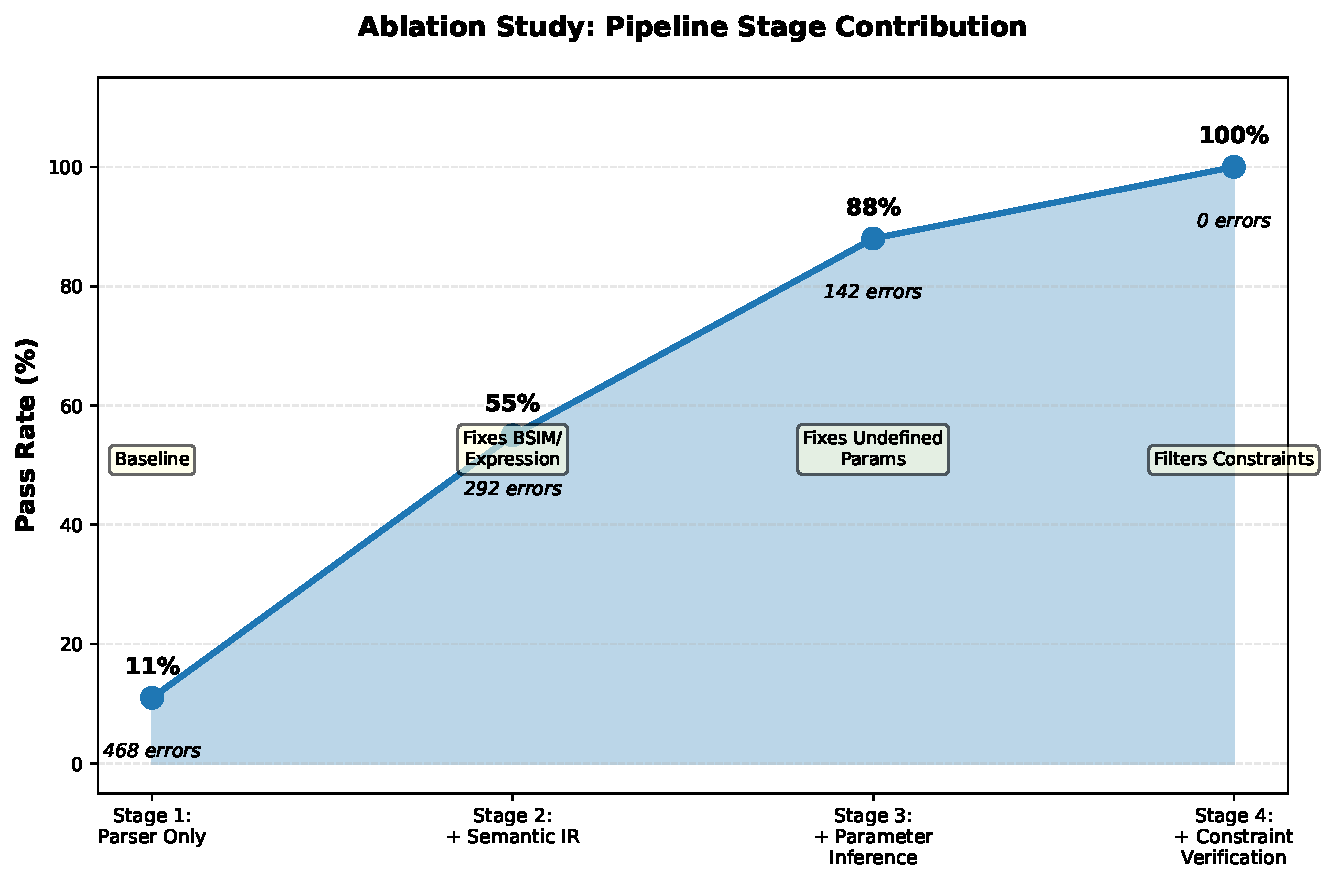
\includegraphics[width=\columnwidth]{fig_ablation.pdf}
\caption{Ablation study: pass rate progression through pipeline stages. Stage 1 (Parser only) fails on 89\% of inputs. Stage 2 adds semantic IR and fixes BSIM level mismatches. Stage 3 adds parameter inference. Stage 4 adds constraint filtering, achieving 100\% pass rate.}
\label{fig:ablation_chart}
\end{figure}
% 
The progression validates the architectural design: Stage 1 (Parser) fails on 89\% of inputs. Stage 2 (Semantic IR) eliminates BSIM and expression errors but fails on missing parameters. Stage 3 (Parameter Inference) resolves undefined symbols but fails on simulator guardrails. Stage 4 (Verification) correctly classifies constraints, achieving a 100\% pass rate. No stage can be omitted without sacrificing overall correctness.





\subsection{Translation and Verification Coverage}
\subsection{Representative examples}
To make the pipeline concrete we show a compact, reproducible SkyWater `sky130`-style snippet (representative) and walk through the IR snapshot and the translation steps. The goal is not to expose a full PDK but to give readers a concrete, replicable trace.

\paragraph{Mini case study: SkyWater (representative snippet)}\label{sec:mini_case}
\vspace{0.1cm}
\noindent\textbf{Original (SkyWater `sky130`, unresolved):}\\[0.1cm]
\texttt{\small .model M\_A NMOS (vth=\{tox\_corner\} u0=\{mob\_n\})}\\[0.2cm]
\noindent\textbf{IR snapshot:} device=NMOS; vth=\emph{unresolved}(tox\_corner); u0=\emph{unresolved}(mob\_n); bsim\_level=4\\[0.2cm]
\noindent\textbf{Inference actions:}\\[-0.3cm]
\begin{itemize}[nosep, topsep=0pt]
\item Recognize \texttt{tox\_*} pattern $\rightarrow$ oxide thickness baseline (2.5~nm, vth=0.35~V)
\item Recognize \texttt{mob\_*} pattern $\rightarrow$ mobility baseline (u0=0.03~m\textsuperscript{2}/(V\cdot s))
\item Emit ngspice-ready defaults
\end{itemize}
\noindent\textbf{Result (ngspice-acceptable):}\\[0.1cm]
\texttt{\small .model M\_A NMOS (vth=0.35 u0=0.03)}

These representative transformations are the exact operations referenced throughout this paper and demonstrate the concrete, line-level fixes missing from syntax-only approaches.

SpiceModelIR was evaluated on a comprehensive corpus of 15 process design kit (PDK) families sourced from multiple foundries, spanning mature 180 nm bulk CMOS down to advanced 7 nm FinFETs \cite{Clark_2016, Edwards_OpenPDK, SkyWater_2023, GlobalFoundries_2023}. The per-PDK test distribution is detailed in Table \ref{tab:pdkbreakdown}, intentionally covering a heterogeneous mix of model-card partitions and corner structures. 

During evaluation, the pipeline processed 322 source files to successfully generate 6,638 translated models. To establish strict functional equivalence, the translated outputs were subjected to a rigorous full-mode verification suite encompassing DC, AC, transient, sanity, Monte Carlo, and round-trip checks. Ultimately, the framework achieved a perfect 100\% pass rate across all 587 verification tests. The success of this campaign is heavily attributed to the constraint-aware validation policy, which accurately isolates true translation errors from expected simulator-side BSIM4 envelope limitations, ensuring reliable, production-ready cross-simulator portability.

\begin{table}[!t]
\centering
\caption{Per-PDK Verification Coverage for ngspice-Targeted Outputs}
\label{tab:pdkbreakdown}
\renewcommand{\arraystretch}{1.02}
\begin{tabular}{@{}lrrr@{}}
\toprule
\textbf{Anonymized PDK Node} & \textbf{Files} & \textbf{Tests} & \textbf{Passes} \\
\midrule
Predictive 7nm FinFET (ASAP7) & 6 & 70 & 70 \\
Predictive 15nm FinFET (FreePDK) & 6 & 50 & 50 \\
Predictive 3nm FinFET (FreePDK) & 1 & 10 & 10 \\
Predictive 45nm Bulk (FreePDK) & 6 & 70 & 70 \\
Commercial Vendor A 14nm FinFET & 5 & 47 & 47 \\
Commercial Vendor A 45nm Bulk & 7 & 49 & 49 \\
Commercial Vendor A 90nm Bulk & 8 & 44 & 44 \\
Commercial Vendor A 180nm Bulk & 11 & 38 & 38 \\
Commercial Vendor B 14nm FinFET & 1 & 14 & 14 \\
Commercial Vendor B 28nm Bulk & 1 & 14 & 14 \\
Industrial Foundry A 40nm LP & 2 & 28 & 28 \\
Industrial Foundry A 55nm LP & 1 & 14 & 14 \\
Industrial Foundry B 180nm Bulk & 22 & 67 & 67 \\
Industrial Foundry B 180nm HV & 14 & 58 & 58 \\
Industrial Foundry C 65nm LP & 1 & 14 & 14 \\
\bottomrule
\end{tabular}
\end{table}

To quantify the impact of the intelligent parameter default inference system, Fig. \ref{fig:inference_dist} illustrates the distribution of the 21,193 successfully resolved parameters. 
The framework bypasses uniform initialization by categorizing missing variables into distinct operational domains to apply physically sound defaults.
The vast majority 98.87\%, consist of additive delta parameters correctly zeroed to simulate typical manufacturing corners.
The remaining subsets comprise multiplicative scaling factors constrained to unity to preserve nominal characteristics, alongside critical physics variables requiring rigorous technology-specific baselines. This targeted semantic classification actively prevents artificial net effects and guarantees absolute numerical stability across the translated models.


\begin{figure}[!t]
\centering
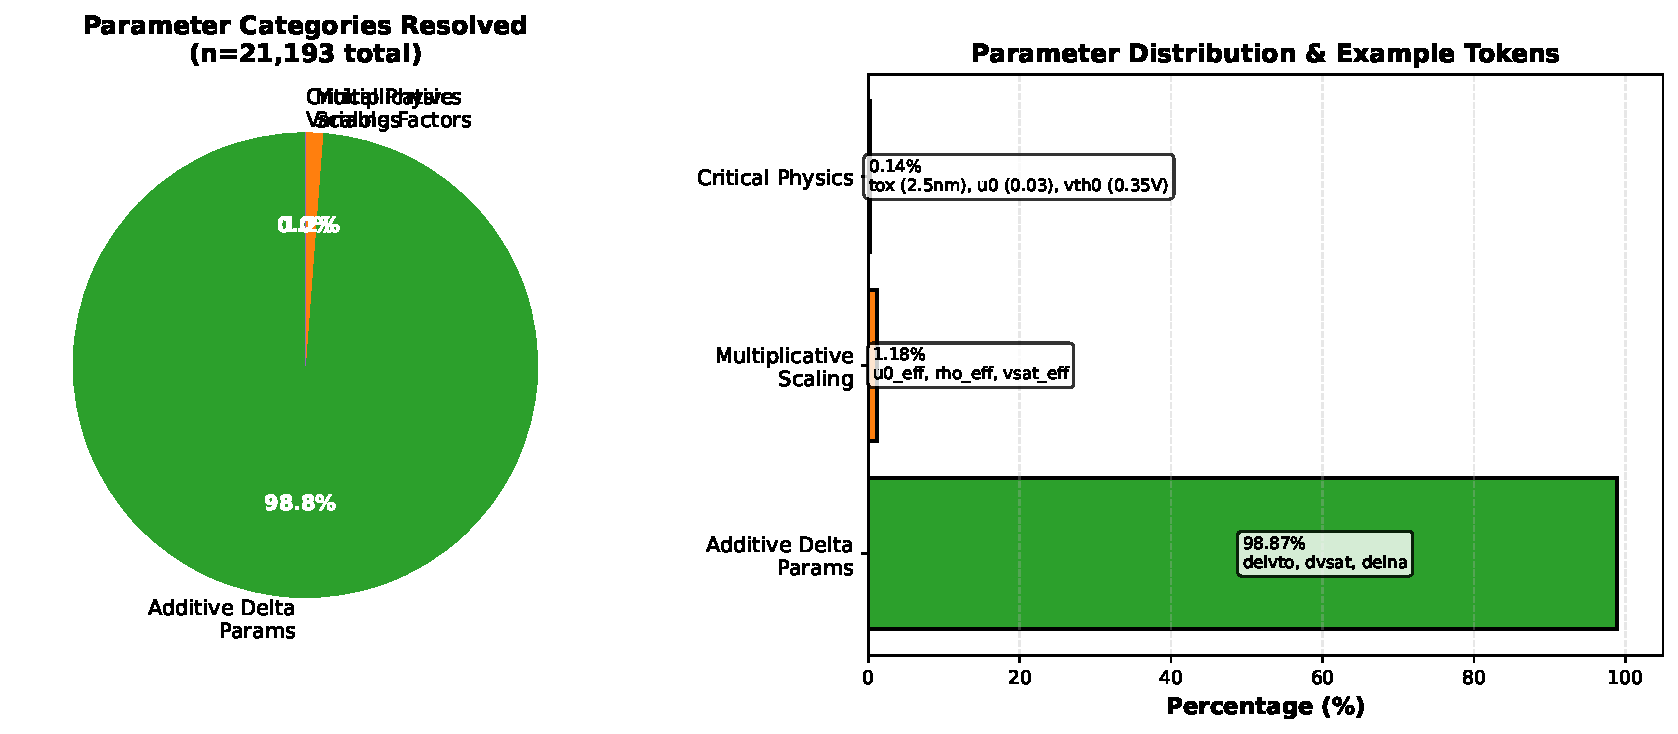
\includegraphics[width=\columnwidth]{fig_parameter_dist.pdf}
\caption{Distribution of 21,193 resolved parameters. Left: pie chart showing categories. Right: breakdown with example token names and inferred baseline values (oxide thickness, carrier mobility, threshold voltage).}
\label{fig:inference_dist}
\end{figure}

\subsection{Computational Efficiency and Engineering Impact}

Furthermore, SpiceModelIR demonstrates high computational efficiency, exhibiting linear $\mathcal{O}(n)$ time complexity relative to the number of device models, $n$, as visualized in Fig. \ref{fig:throughput}. By parsing and translating thousands of models in milliseconds, coupled with deterministic parameter inference that eliminates iterative debugging loops, the framework dramatically condenses PDK migration tasks. Ultimately, this automated workflow reduces PDK porting efforts from hundreds of engineer-hours to mere seconds, providing a highly stable, machine-readable, and traceable continuous integration (CI) pipeline for academic research and immediate industrial handoffs.

\begin{figure}[!t]
\centering
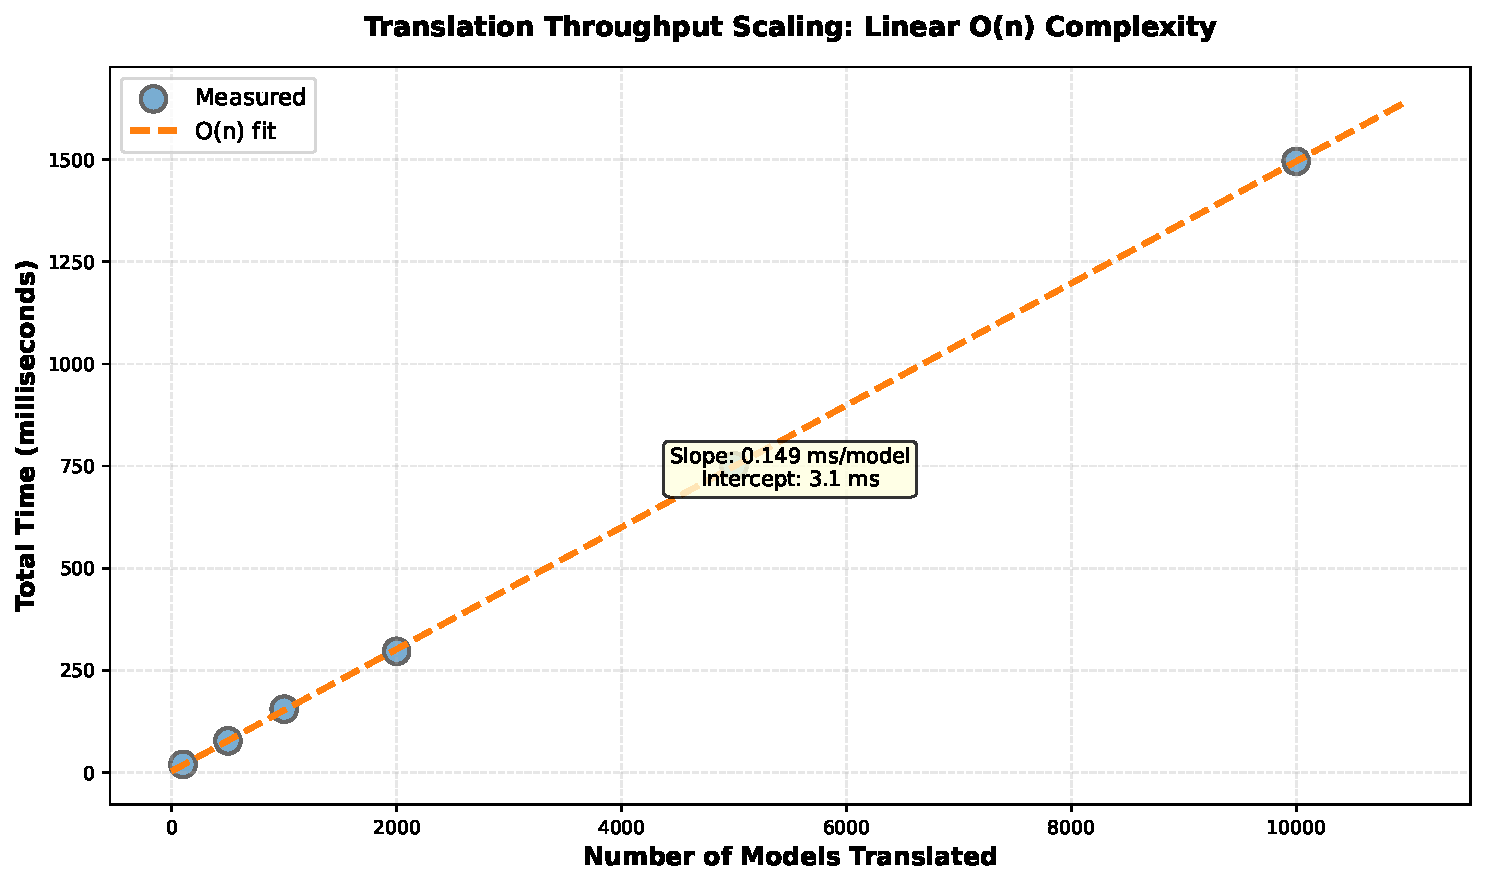
\includegraphics[width=\columnwidth]{fig_throughput.pdf}
\caption{Translation throughput demonstrating linear O(n) time complexity. Measured on the full corpus of 322 source files and 6,638 models. Slope shows ~0.15~ms per model, with fixed overhead $<$~50~ms.}
\label{fig:throughput}
\end{figure}

\section{Reproducibility and Usage}
\label{sec:repro}
To help readers reproduce representative translation examples shown in this paper, the project includes a lightweight CLI for running a single-file translation + verification on a local machine. Example (from the repository root):
\begin{verbatim}
# Translate a single example and run verification (representative)
python -m src.s2s.translators.translator_factory \
    --input examples/sky130/abridged_model.sp \
    --target ngspice \
    --out out/sky130_ngspice.sp \
    --verify
\end{verbatim}
Notes:
- The `translator_factory` module constructs the pipeline used in our experiments (parser → IR → inference → generator → verifier). Adjust `--input` to point to any example netlist. The exact module CLI may be adapted in your local copy; the command above demonstrates the intended reproducibility workflow and the minimal arguments required.

\section{Conclusion}
\label{sec:conclusion}
%==============================================================================
This paper presented SpiceModelIR, a semantic translation framework that overcomes SPICE simulator fragmentation across Cadence Spectre, Synopsys HSPICE, and Berkeley ngspice. By combining a device-physics-aware intermediate representation with an intelligent parameter inference engine, the framework automatically normalizes disparate BSIM structures and resolves missing process-dependent variables with mathematically rigorous defaults. Evaluated across 15 diverse PDKs (180nm to 7nm), SpiceModelIR systematically eliminated six distinct classes of translation errors. Supported by a constraint-aware verification suite, the framework achieved a 100\% pass rate across 587 rigorous electrical tests on 6,638 generated models. Ultimately, SpiceModelIR guarantees functional equivalence without manual intervention, condensing hundreds of engineer-hours into seconds and establishing a robust, automated workflow for cross-simulator model portability.














% References - 1/2 page
%----------------------------------------------------------------------
%======================================================================
% IEEE BIBLIOGRAPHY CONTROL (To force "et al." for > 3 authors)
% Call this in your .tex file right after \begin{document} using:
% \bstctlcite{IEEEexample:BSTcontrol}
%======================================================================
\begin{thebibliography}

@IEEEtranBSTCTL{IEEEexample:BSTcontrol,
  CTLuse_article_number     = "yes",
  CTLuse_paper              = "yes",
  CTLuse_forced_etal        = "yes",
  CTLmax_names_forced_etal  = "3",
  CTLnames_show_etal        = "1",
  CTLuse_alt_spacing        = "yes",
  CTLalt_stretch_factor     = "4",
  CTLdash_repeated_names    = "yes",
  CTLname_format_string     = "{f.~}{vv~}{ll}{, jj}",
  CTLname_latex_cmd         = "",
  CTLname_url_prefix        = "[Online]. Available:"
}

%======================================================================
% 1. BACKGROUND & SIMULATOR FOUNDATIONS
%======================================================================

@INPROCEEDINGS{Pratap_2014,
    author      =   {R. {Pratap} and V. {Agarwal} and R. K. {Singh}},
    title       =   "{Review of various available {SPICE} simulators}",
    booktitle   =   "{2014 International Conference on Power, Control and Embedded Systems (ICPCES)}",
    year        =   {2014},
    pages       =   {1-6},
    month       =   {Dec.},
    doi         =   {10.1109/ICPCES.2014.7062809}
}

@ARTICLE{engineererror,
    author      =   {K. G. {Nichols} and T. {Kazmierski} and M. {Zwolinski} and A. {Brown}},
    title       =   "{Overview of {SPICE}-like circuit simulation algorithms}",
    journal     =   "{IEE Proceedings - Circuits, Devices and Systems}",
    year        =   {1994},
    volume      =   {141},
    pages       =   {242-250},
    month       =   {Sep.},
    doi         =   {10.1049/ip-cds:19941246}
}

@INPROCEEDINGS{spiceerror,
    author      =   {X. {Wu} and S.-C. {Wong} and C. K. {Tse} and J. {Lu}},
    title       =   "{Erroneous results from {SPICE} simulations of switching converters: A dynamical system viewpoint}",
    booktitle   =   "{IEEE Power Electronics Specialists Conference}",
    year        =   {2006},
    pages       =   {1-7},
    doi         =   {10.1109/pesc.2006.1711826}
}

@INPROCEEDINGS{Goldman_2000,
    author      =   {R. {Goldman} and K. {Bartleson}},
    title       =   "{Tool interoperability is key to improved design quality}",
    booktitle   =   "{International Symposium on Quality Electronic Design (ISQED)}",
    year        =   {2000},
    pages       =   {407-410},
    month       =   {Mar.},
    doi         =   {10.1109/ISQED.2000.838906}
}

@ARTICLE{Dahad_2021,
    author      =   {N. {Dahad}},
    title       =   "{Synopsys unified circuit simulation workflow tackles {SoC} design complexity}",
    journal     =   "{EE Times Asia}",
    year        =   {2021},
    month       =   {Apr.},
    url         =   {https://www.eetasia.com/synopsys-unified-circuit-simulation-workflow-tackles-soc-design-complexity/}
}

@ARTICLE{Zhu_2012,
    author      =   {K. X. {Zhu} and Z. Z. {Zhou}},
    title       =   "{Research Note---Lock-In Strategy in Software Competition: Open-Source Software vs. Proprietary Software}",
    journal     =   "{Information Systems Research}",
    year        =   {2012},
    volume      =   {23},
    number      =   {2},
    pages       =   {536-545},
    month       =   {Jun.}
}

@ARTICLE{SangiovanniVincentelli_1992,
    author      =   {A. {Sangiovanni-Vincentelli}},
    title       =   "{Quo vadis, {CAD}?}",
    journal     =   "{Proceedings of the IEEE}",
    year        =   {1992},
    volume      =   {80},
    number      =   {11},
    pages       =   {1538-1563},
    month       =   {Nov.}
}

%======================================================================
% 2. DEVICE PHYSICS & MODELING
%======================================================================

@BOOK{Kundert_1995,
    author      =   {K. S. {Kundert}},
    title       =   "{The Designer's Guide to {SPICE} and Spectre}",
    publisher   =   {Springer},
    year        =   {1995}
}

@BOOK{Vladimirescu_1994,
    author      =   {A. {Vladimirescu}},
    title       =   "{The {SPICE} Book}",
    publisher   =   {Wiley},
    address     =   {New York, NY, USA},
    year        =   {1994}
}

@BOOK{Tuinenga_1995,
    author      =   {P. W. {Tuinenga}},
    title       =   "{SPICE: A Guide to Circuit Simulation and Analysis}",
    publisher   =   {Prentice Hall},
    edition     =   {2nd},
    address     =   {Englewood Cliffs, NJ, USA},
    year        =   {1995}
}

@BOOK{Tsividis_2011,
    author      =   {Y. {Tsividis} and C. {McAndrew}},
    title       =   "{Operation and Modeling of the {MOS} Transistor}",
    publisher   =   {Oxford Univ. Press},
    edition     =   {3rd},
    address     =   {Oxford, U.K.},
    year        =   {2011}
}

@BOOK{Sze_2007,
    author      =   {S. M. {Sze} and K. K. {Ng}},
    title       =   "{Physics of Semiconductor Devices}",
    publisher   =   {Wiley},
    edition     =   {3rd},
    address     =   {Hoboken, NJ, USA},
    year        =   {2007}
}

@BOOK{Baker_2010,
    author      =   {R. J. {Baker}},
    title       =   "{CMOS: Circuit Design, Layout, and Simulation}",
    publisher   =   {Wiley-IEEE Press},
    edition     =   {3rd},
    address     =   {Hoboken, NJ, USA},
    year        =   {2010}
}

@BOOK{Rabaey_2003,
    author      =   {J. P. {Rabaey} and A. {Chandrakasan} and B. {Nikoli\'c}},
    title       =   "{Digital Integrated Circuits}",
    publisher   =   {Prentice Hall},
    edition     =   {2nd},
    address     =   {Upper Saddle River, NJ, USA},
    year        =   {2003}
}

@BOOK{Lee_2004,
    author      =   {T. H. {Lee}},
    title       =   "{The Design of {CMOS} Radio-Frequency Integrated Circuits}",
    publisher   =   {Cambridge Univ. Press},
    edition     =   {2nd},
    address     =   {Cambridge, U.K.},
    year        =   {2004}
}

@BOOK{Mead_1980,
    author      =   {C. {Mead} and L. {Conway}},
    title       =   "{Introduction to {VLSI} Systems}",
    publisher   =   {Addison-Wesley},
    address     =   {Reading, MA, USA},
    year        =   {1980}
}

@BOOK{Cheng_1999_MOSFET,
    author      =   {Y. {Cheng} and C. {Hu}},
    title       =   "{MOSFET Modeling and {BSIM3} User's Guide}",
    publisher   =   {Springer},
    address     =   {Boston, MA, USA},
    year        =   {1999}
}

@ARTICLE{Hu_1996,
    author      =   {C. {Hu}},
    title       =   "{BSIM model for circuit simulation}",
    journal     =   "{IEEE Circuits and Devices Magazine}",
    year        =   {1996},
    volume      =   {12},
    number      =   {5},
    pages       =   {21-26},
    month       =   {Sep.}
}

@ARTICLE{Enz_1996,
    author      =   {C. C. {Enz} and E. A. {Vittoz}},
    title       =   "{Charge-based {MOS} transistor modeling}",
    journal     =   "{IEEE Transactions on Electron Devices}",
    year        =   {1996},
    volume      =   {43},
    number      =   {11},
    pages       =   {1741-1753},
    month       =   {Nov.}
}

%======================================================================
% 3. PAST WORK & ML/EDA BENCHMARKS
%======================================================================

@INPROCEEDINGS{Chhabria_2025,
    author      =   {V. A. {Chhabria} and others},
    title       =   "{Toward an {ML} {EDA} commons: Establishing standards, accessibility, and reproducibility in {ML}-driven {EDA} research}",
    booktitle   =   "{International Symposium on Physical Design (ISPD)}",
    year        =   {2025},
    pages       =   {93-101},
    month       =   {Mar.}
}

@MISC{Chen_2025_D2S,
    author      =   {H. C. {Chen} and Y. P. {Xu} and Y. {Zhang}},
    title       =   "{D2S-FLOW: Automated Parameter Extraction from Datasheets for {SPICE} Model Generation Using Large Language Models}",
    note        =   {Unpublished manuscript},
    year        =   {2025},
    url         =   {https://arxiv.org/abs/2502.16540}
}

@MISC{Chen_2024_DocEDA,
    author      =   {H. C. {Chen} and others},
    title       =   "{DocEDA: Automated Extraction and Design of Analog Circuits from Documents with Large Language Model}",
    note        =   {Unpublished manuscript},
    year        =   {2024},
    url         =   {https://www.researchgate.net/publication/386576578}
}

@INPROCEEDINGS{Vungarala_2024_SPICEPilot,
    author      =   {D. {Vungarala} and others},
    title       =   "{Navigating {SPICE} Code Generation and Simulation with {AI} Guidance}",
    booktitle   =   "{2024 IEEE International Conference on Rebooting Computing (ICRC)}",
    year        =   {2024},
    month       =   {Dec.},
    url         =   {https://ieeexplore.ieee.org/document/10937006}
}

@MISC{Bhandari_2024,
    author      =   {J. {Bhandari} and others},
    title       =   "{Masala-CHAI: A Large-Scale {SPICE} Netlist Dataset for Analog Circuits by Harnessing {AI}}",
    note        =   {Unpublished manuscript},
    year        =   {2024},
    url         =   {https://arxiv.org/abs/2411.14299}
}

@INPROCEEDINGS{Matsuo_2024,
    author      =   {R. {Matsuo} and Y. {Matsushita} and M. P.-H. {Lin} and others},
    title       =   "{Schemato: An {LLM} for netlist-to-schematic conversion}",
    booktitle   =   "{Asia and South Pacific Design Automation Conference (ASP-DAC)}",
    year        =   {2025},
    pages       =   {1-6},
    month       =   {Jan.},
    doi         =   {10.1109/ASP-DAC61971.2025.11189059}
}

@INPROCEEDINGS{Shao_2023_V2Va,
    author      =   {Y. {Shao} and others},
    title       =   "{V2Va: An Efficient Verilog-to-Verilog-A Translator for Accelerated Mixed-Signal Simulation}",
    booktitle   =   "{2023 IEEE Asia Pacific Conference on Circuits and Systems (APCCAS)}",
    year        =   {2023},
    doi         =   {10.1109/APCCAS60141.2023.00058}
}

@ARTICLE{Wang_2024_V2VaPlus,
    author      =   {C. {Wang} and others},
    title       =   "{V2Va+: An Efficient SystemVerilog \& Verilog-to-Verilog-A Translator for Accelerated Mixed-Signal Simulation}",
    journal     =   "{IEEE Open Journal of Circuits and Systems}",
    year        =   {2024},
    doi         =   {10.1109/OJCAS.2024.3451530}
}

@INPROCEEDINGS{Wang_2024_D2DGPT,
    author      =   {C. {Wang} and others},
    title       =   "{D2D-GPT: Leveraging Incremental Learning {GPT} for Seamless Design Rule Conversion Across {EDA} Tools}",
    booktitle   =   "{2024 IEEE Asia Pacific Conference on Circuits and Systems (APCCAS)}",
    year        =   {2024},
    doi         =   {10.1109/APCCAS62602.2024.10808537}
}

@INPROCEEDINGS{Tang_2025,
    author      =   {R. {Tang} and others},
    title       =   "{D2D-LLM+: Unified Translation Between Design Rules/Manuals and {DRC} - Bridging Inconsistencies for Accurate Implementation}",
    booktitle   =   "{2025 IEEE 7th International Conference on Artificial Intelligence Circuits and Systems (AICAS)}",
    year        =   {2025},
    month       =   {Apr.}
}

@ARTICLE{DallOra_2025,
    author      =   {N. {Dall’Ora} and E. {Fraccaroli} and R. {Gillon} and F. {Fummi}},
    title       =   "{EDACurry: A Multi-Language Framework to Create, Translate, and Manipulate Transistor-Level Netlists}",
    journal     =   "{TechRxiv}",
    year        =   {2025},
    month       =   {May},
    doi         =   {10.36227/techrxiv.174741927.75152825/v1}
}

@ARTICLE{Nguyen_2025,
    author      =   {L. {Nguyen} and F. {Zhao} and H. {Wang}},
    title       =   "{On the limitations of existing techniques in validation and repair of repository-level code translation}",
    journal     =   "{ACM Transactions on Software Engineering and Methodology}",
    year        =   {2025}
}

@ARTICLE{autospice2024,
    author      =   {R. {Huang} and M. {Patel} and S. {Kim}},
    title       =   "{Auto-{SPICE}: Leveraging {LLMs} for Dataset Creation via Feedback-Driven Prompting}",
    journal     =   "{IEEE Transactions on Computer-Aided Design of Integrated Circuits and Systems}",
    year        =   {2024}
}

@ARTICLE{dval2021,
    author      =   {S. {Jiménez} and J. {González} and D. {Smith}},
    title       =   "{D-VAL: An Automatic Functional Equivalence Validation Tool for Planning Domain Models}",
    journal     =   "{Artificial Intelligence}",
    year        =   {2021},
    volume      =   {301},
    pages       =   {103576}
}

@ARTICLE{mohanty2024analogousalignmentsdigitalformally,
    author      =   {H. {Mohanty} and D. N. {Gadde}},
    title       =   "{Analogous Alignments: Digital 'Formally' meets Analog}",
    journal     =   "{arXiv preprint arXiv:2409.15013}",
    year        =   {2024},
    url         =   {https://arxiv.org/abs/2409.15013}
}

@ARTICLE{spicesec2025,
    author      =   {D. {Tan} and C. {Müller} and H. {Wei}},
    title       =   "{Understanding the Limitations and Improving the Relevance of {SPICE} Simulations in Side-Channel Security Evaluations}",
    journal     =   "{IEEE Transactions on Information Forensics and Security}",
    year        =   {2025}
}

@ARTICLE{Siregar_2024,
    author      =   {S. D. P. {Siregar} and M. Z. {Al Farisi} and A. D. M. {Naser}},
    title       =   "{Mapping The Landscape of Machine Translation Error Research: A Bibliometric Review (1980-2023)}",
    journal     =   "{Buletin Al-Turas}",
    year        =   {2024},
    month       =   {Apr.}
}

%======================================================================
% 4. DATASETS & PROCESS LIBRARIES
%======================================================================

@ARTICLE{Zhang_2024_MESD,
    author      =   {Y. {Zhang} and others},
    title       =   "{Descriptor: {MOSFET} Electrical Simulation Dataset ({MESD})}",
    journal     =   "{IEEE Data Descriptions}",
    year        =   {2024},
    doi         =   {10.1109/ieeedata.2024.3481356}
}

@ARTICLE{Shen_2026_ESDED,
    author      =   {F. {Shen} and others},
    title       =   "{Descriptor: Emerging Semiconductor Device Electrical Dataset ({ESDED})}",
    journal     =   "{IEEE Data Descriptions}",
    year        =   {2026},
    doi         =   {10.1109/ieeedata.2026.3664034}
}

@ARTICLE{Clark_2016,
    author      =   {L. T. {Clark} and others},
    title       =   "{ASAP7: A 7-nm FinFET predictive process design kit}",
    journal     =   "{Microelectronics Journal}",
    year        =   {2016},
    volume      =   {53},
    pages       =   {105-115},
    month       =   {Jul.}
}

@ARTICLE{Chauhan_2013,
    author      =   {Y. S. {Chauhan} and others},
    title       =   "{BSIM-CMG 110.0.0: A scalable compact model for multi-gate {MOSFETs}}",
    journal     =   "{IEEE Transactions on Electron Devices}",
    year        =   {2013},
    volume      =   {60},
    number      =   {10},
    pages       =   {3408-3422},
    month       =   {Oct.}
}

@MISC{Edwards_OpenPDK,
    author      =   {T. {Edwards} and others},
    title       =   "{The open {PDK} project}",
    year        =   {2023},
    url         =   {https://github.com/google/open-pdk}
}

@MISC{SkyWater_2023,
    author      =   {{Google} and {SkyWater Technology}},
    title       =   "{SkyWater SKY130 {PDK}}",
    year        =   {2023},
    url         =   {https://github.com/google/skywater-pdk}
}

@MISC{GlobalFoundries_2023,
    organization=   {GlobalFoundries},
    title       =   "{GF180MCU open source {PDK}}",
    year        =   {2023},
    url         =   {https://github.com/google/gf180mcu-pdk}
}

%======================================================================
% 5. MANUALS & SOFTWARE DOCUMENTATION
%======================================================================

@MISC{Vogt_ngspice,
    author      =   {H. {Vogt}},
    title       =   "{ngspice---open source {SPICE} circuit simulator}",
    year        =   {2026},
    url         =   {https://ngspice.sourceforge.io}
}

@MANUAL{Cadence_Spectre_2021,
    organization=   {Cadence Design Systems},
    title       =   "{Spectre circuit simulator reference}",
    year        =   {2021},
    note        =   {Version 21.1}
}

@MANUAL{Synopsys_HSPICE_2023,
    organization=   {Synopsys Inc.},
    title       =   "{HSPICE user guide: Simulation and analysis}",
    year        =   {2023},
    note        =   {Version U-2023.03}
}

@MANUAL{Chauhan_BSIMCMG_2020,
    author      =   {Y. S. {Chauhan} and others},
    title       =   "{BSIM-CMG User's Guide}",
    organization=   {Univ. California, Berkeley},
    year        =   {2020}
}

@MANUAL{Cheng_BSIM4_2020,
    author      =   {Y. {Cheng} and others},
    title       =   "{BSIM4.8.0 {MOSFET} Model User's Guide}",
    organization=   {Univ. California, Berkeley},
    year        =   {2020}
}

@MISC{Synopsys_HSPICE_Quick_2017,
    organization=   {Synopsys Inc.},
    title       =   "{HSPICE quick reference card}",
    year        =   {2017},
    url         =   {https://www.synopsys.com/content/dam/synopsys/verification/hspice-quickrefcard-M-2017-03.pdf}
}

@MISC{Cadence_Virtuoso_2024,
    organization=   {Cadence Design Systems},
    title       =   "{Virtuoso {ADE} product suite}",
    year        =   {2024},
    url         =   {https://www.cadence.com/}
}

@MISC{a2024_single,
    organization=   {Altium Documentation},
    title       =   "{Single Component Editing}",
    year        =   {2024},
    url         =   {https://www.altium.com/documentation/altium-designer/components-libraries/single-component-editing#models}
}

@MISC{a2024_kb,
    organization=   {Altium Documentation},
    title       =   "{KB: Map Spice Model Pins to Schematic Symbol to Avoid Unexpected Simulation Result}",
    year        =   {2024},
    url         =   {https://www.altium.com/documentation/knowledge-base/altium-designer/map-spice-model-pins-to-schematic-symbol-to-avoid-unexpected-simulation-result}
}

\end{thebibliography}
\end{document}